\documentclass[12pt]{article}

\title{SCL Example Robot : RPP Bot}      
\author{Samir Menon, smenon@stanford.edu}

\usepackage{graphicx}
\usepackage[top=2cm, bottom=3cm, left=1.5cm, right=1.5cm]{geometry}
%For stretching tables.
\usepackage{tabularx}

\usepackage{amssymb,amsmath}

\begin{document}
\maketitle


\begin{figure}[ht!]
\begin{center}
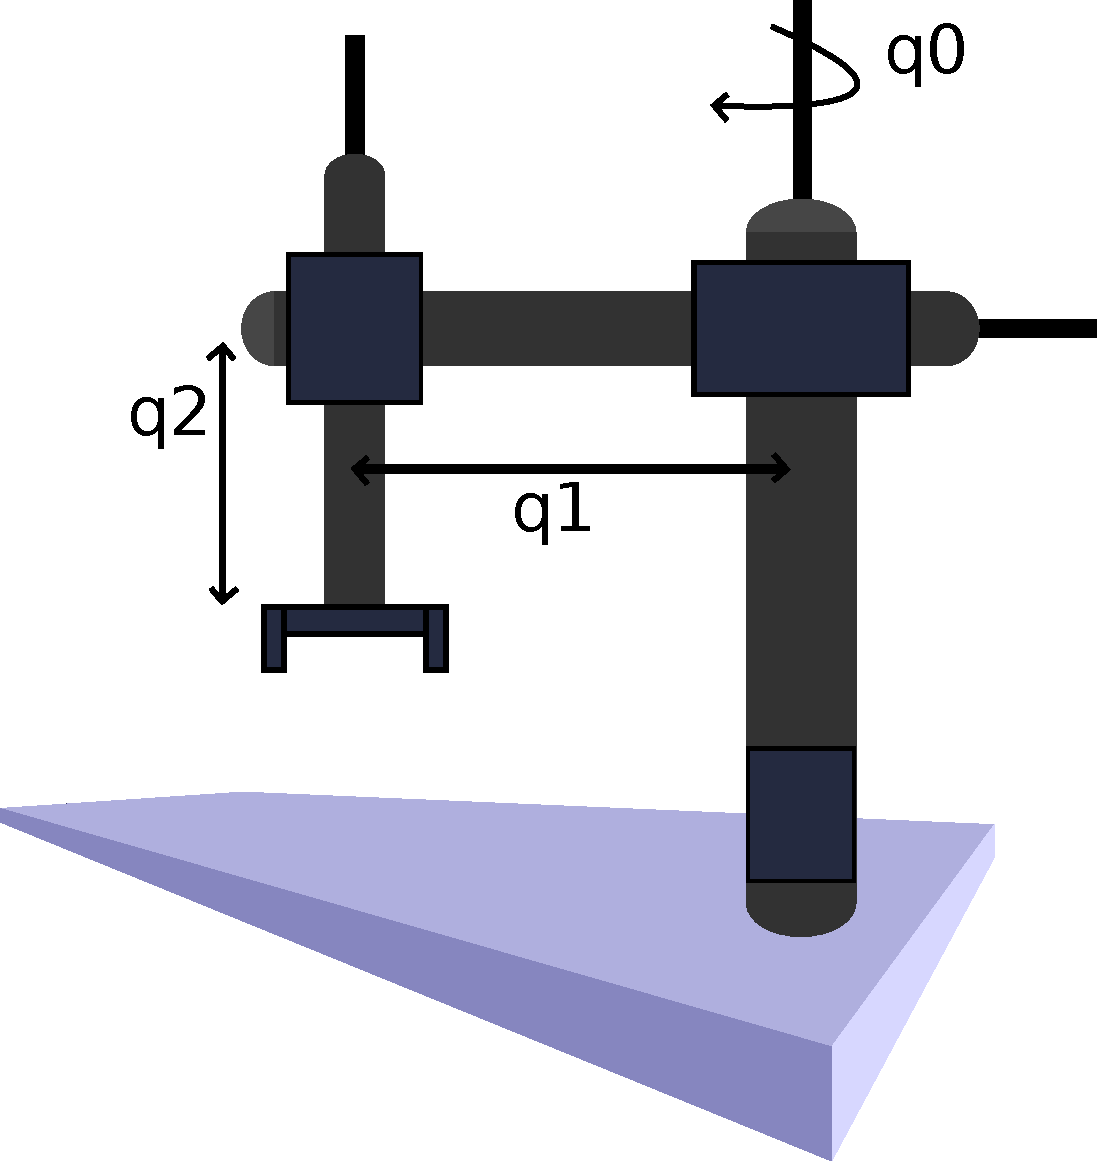
\includegraphics[width=4in]{figs/rpp.pdf}
\caption{RPP Bot schematic}
\label{fig:rppbot}
\end{center}
\end{figure}


\section{Description}
RPP is a revolute-prismatic-prismatic robot (Fig. \ref{fig:rppbot}) built to
demonstrate control and dynamics. It is a simple robot whose dynamics can be
computed analytically.

\begin{figure}[ht!]
\begin{center}
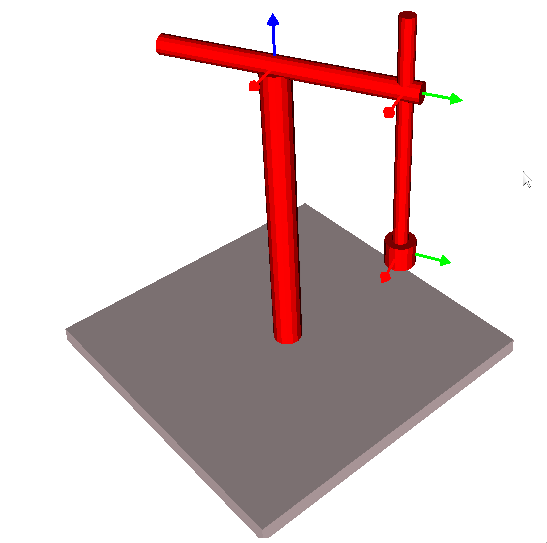
\includegraphics[width=4in]{figs/rpp-bot-frames.png}
\caption{RPP Bot Frames: Frame$_0$ rotates with $q_0$ about the z-axis, frame$_1$ moves along the y-axis 
with $q_1$ and frame$_2$ moves along the z-axis with $q_2$. The x, y and z axes are colored red, green 
and blue respectively. Each frame has an offset given in the transformation equations.}
\label{fig:rppframes}
\end{center}
\end{figure}

\section{Kinematic Transformations}
The kinematic transformations are useful to transform the motion of a point on the robot
from link-centric coordinates to global coordinates. Trajectories are usually specified in
fixed global coordinates (it is much easier to do so) and a controller can use the kinematics to
compute an error between the position of a point on the robot and the trajectory in global
coordinates.

The robot is connected to a ground frame (-1). Its base frame (frame$_0$) is computed
from the ground frame after a rotation about $q_0$ and a translation up to the
point where link$_0$ connects to link$_1$. Thus, frame$_0$ rotates with link$_0$.
Next, link$_1$ moves along the y-axis, and link$_2$ moves along the z-axis (Fig. \ref{fig:rppframes}).
Offsets for frames 0, 1 and 2 are given by $l_0$, $l_1$ and $l_2$ respectively. Frame$_2$ is at the
end-effector.

The transformation matrices are given by:
\begin{equation}
  ^{-1} T_{0} = 
  \begin{bmatrix} 
  cos(q_0) & -sin(q_0) & 0 & 0 \\ 
  sin(q_0) & cos(q_0) & 0 & 0 \\
  0 & 0 & 1 & l_{0} \\
  0 & 0 & 0 & 1 
  \end{bmatrix}
\end{equation}

\begin{equation}
  ^0 T_{1} = 
  \begin{bmatrix} 
  1 & 1 & 0 & 0 \\ 
  0 & 1 & 0 & q_1+l_{1} \\
  0 & 0 & 1 & 0 \\
  0 & 0 & 0 & 1 
  \end{bmatrix}
\end{equation}

\begin{equation}
  ^1 T_{2} = 
  \begin{bmatrix} 
  1 & 1 & 0 & 0 \\ 
  0 & 1 & 0 & 0 \\
  0 & 0 & 1 & q_2+l_{2} \\
  0 & 0 & 0 & 1 
  \end{bmatrix}
\end{equation}

And any vector may be transformed from the end-effector frame to the ground
frame by the following transformation:

\begin{equation}
  ^{ground-frame} v =  ^{-1} T_0 * ^0 T_1 * ^1 T_2 * ^{end-effector-frame} v
\end{equation}

One may similarly construct the inverse transformations from the ground to the end-effector.

\section{Jacobian}
The Jacobian relates the velocity at the a given cartesian point (the operational point)
 to the velocity of the joints.
\begin{equation}
  \dot x = J * \dot q
\end{equation}

For this RPP robot we have:
\begin{equation}
  \begin{bmatrix} 
  \dot x \\
  \dot y \\
  \dot z \\
  \end{bmatrix} 
  = 
  {\Large
  \begin{bmatrix} 
    \frac{\delta x}{\delta q_0} & \frac{\delta x}{\delta q_1} & \frac{\delta x}{\delta q_2} \\
    \\
    \frac{\delta y}{\delta q_0} & \frac{\delta y}{\delta q_1} & \frac{\delta y}{\delta q_2} \\ 
    \\
    \frac{\delta z}{\delta q_0} & \frac{\delta z}{\delta q_1} & \frac{\delta z}{\delta q_2}
  \end{bmatrix} 
  }* 
  \begin{bmatrix}
  \dot q_0 \\
  \dot q_1 \\
  \dot q_2 
  \end{bmatrix} 
\end{equation}

The end-effector is a natural operational point since the robot must move it around to do 
tasks. Computing its Jacobian, however, requires moving to ground coordinates first (that's
where the trajectory is specified). For this simple robot, we can get the Jacobian analytically by 
computing\\ $^{ground-frame}$x$_{end-effector-frame}$
\begin{equation}
  x = -(q_1 + l_1) * sin(q_0)
\end{equation}
\begin{equation}
  y = (q_1 + l_1) * cos(q_0)
\end{equation}
\begin{equation}
  z = (l_0+q_2 + l_2),
\end{equation}
 and partially differentiating it with respect to q
\begin{equation}
  J = 
  \begin{bmatrix} 
    -(q_1 + l_1) * cos(q_0) & -sin(q_0) & 0 \\
    \\
    -(q_1 + l_1) * sin(q_0) & cos(q_0) & 0 \\ 
    \\
    0 & 0 & 1
  \end{bmatrix}
\end{equation}

The Jacobian gives us the change in the end-effector's position (in global coordinates) for a small
change in the joint angles. Being able to compute the Jacobian is necessary for dynamic operational
space control. Read on to find out why.

\section{Dynamics}
The robot's dynamics describe the robot's motion characteristics due to its mass and inertia. 
Assuming no external forces (for now), the robot's kinetic energy is given by:
\begin{equation}
  E = \sum_{i=0}^{n-dof} \frac{1}{2} (^{cm}v_i^T * ^{cm} m_i * ^{cm} v_i)
\end{equation}


\section{Operational Space Control}


\end{document}





